\section{Mixture Models \& Secant Varieties}

\begin{frame}{Hidden Variables}
    \begin{itemize}
    \item Suppose $\mc{P} \subset \Delta_{r-1}$ is a model for a random variable $X$ with state space $[r]$.
    \item Moreover, assume that there is a \emph{hidden} or \emph{latent} random variable $Y$ with state space $[s]$, and for each $j \in [s]$, the conditional distribution of $X$ given $Y = j$ is $p^{(j)} \in \mc{P}$. 
    \item The hidden variable $Y$ also has some probability distribution $\pi \in \Delta_{s-1}$.
    \end{itemize}

    So the joint distribution of $Y$ and $X$ is given by the formula
    $$ P(Y = j; X = i) = \pi_{j} \cdot p_{i}^{(j)}. $$

\end{frame}

\begin{frame}{Mixture Models}

    \begin{itemize}
    \item But as $Y$ is hidden, we can only observe the marginal distribution of $X$, that is
    $$ P(X = i) = \sum_{j = 1}^{s} \pi_{j} \cdot p_{i}^{(j)}. $$

    \item In other words, the marginal distribution of $X$ is the convex combination of the $s$ distributions $p^{(1)}, \ldots, p^{(s)}$, with weights given by $\pi$.
    \end{itemize}

    \begin{block}{Definition}
        Let $\mc{P} \subset \Delta_{r-1}$ be a statistical model. The \emph{$s$-th mixture model} is
        $$ \Mixt^{s}(\mc{P}) := \Set{ \sum_{j = 1}^{s} \pi_{j}\cdot p^{(j)} | \pi \in \Delta_{s-1},\ p^{(j)} \in \mc{P}, \text{ for all } j }. $$
    \end{block}

\end{frame}

\begin{frame}{Mixture Models}

    \begin{itemize}
    \item Mixture models provide ways to build complex models out of simpler ones.

    \item Basic assumption is that the underlying population to be modelled can be split into $s$ disjoint sub-populations.

    \item Restricted to each sub-population, the observable $X$ follows a probability distribution from the simple model $\mc{P}$.

    \item After marginalisation though, the structure becomes significantly more complex as it is now a convex combination of these simple distributions.

    \end{itemize}

\end{frame}

\begin{frame}{Phylogenetic Trees}

    \begin{itemize}
        \item Introduce \emph{phylogenetic trees}; describe the descent of species from a common ancestor:        
        \begin{block}{Example Cartoon}

        \begin{center}
        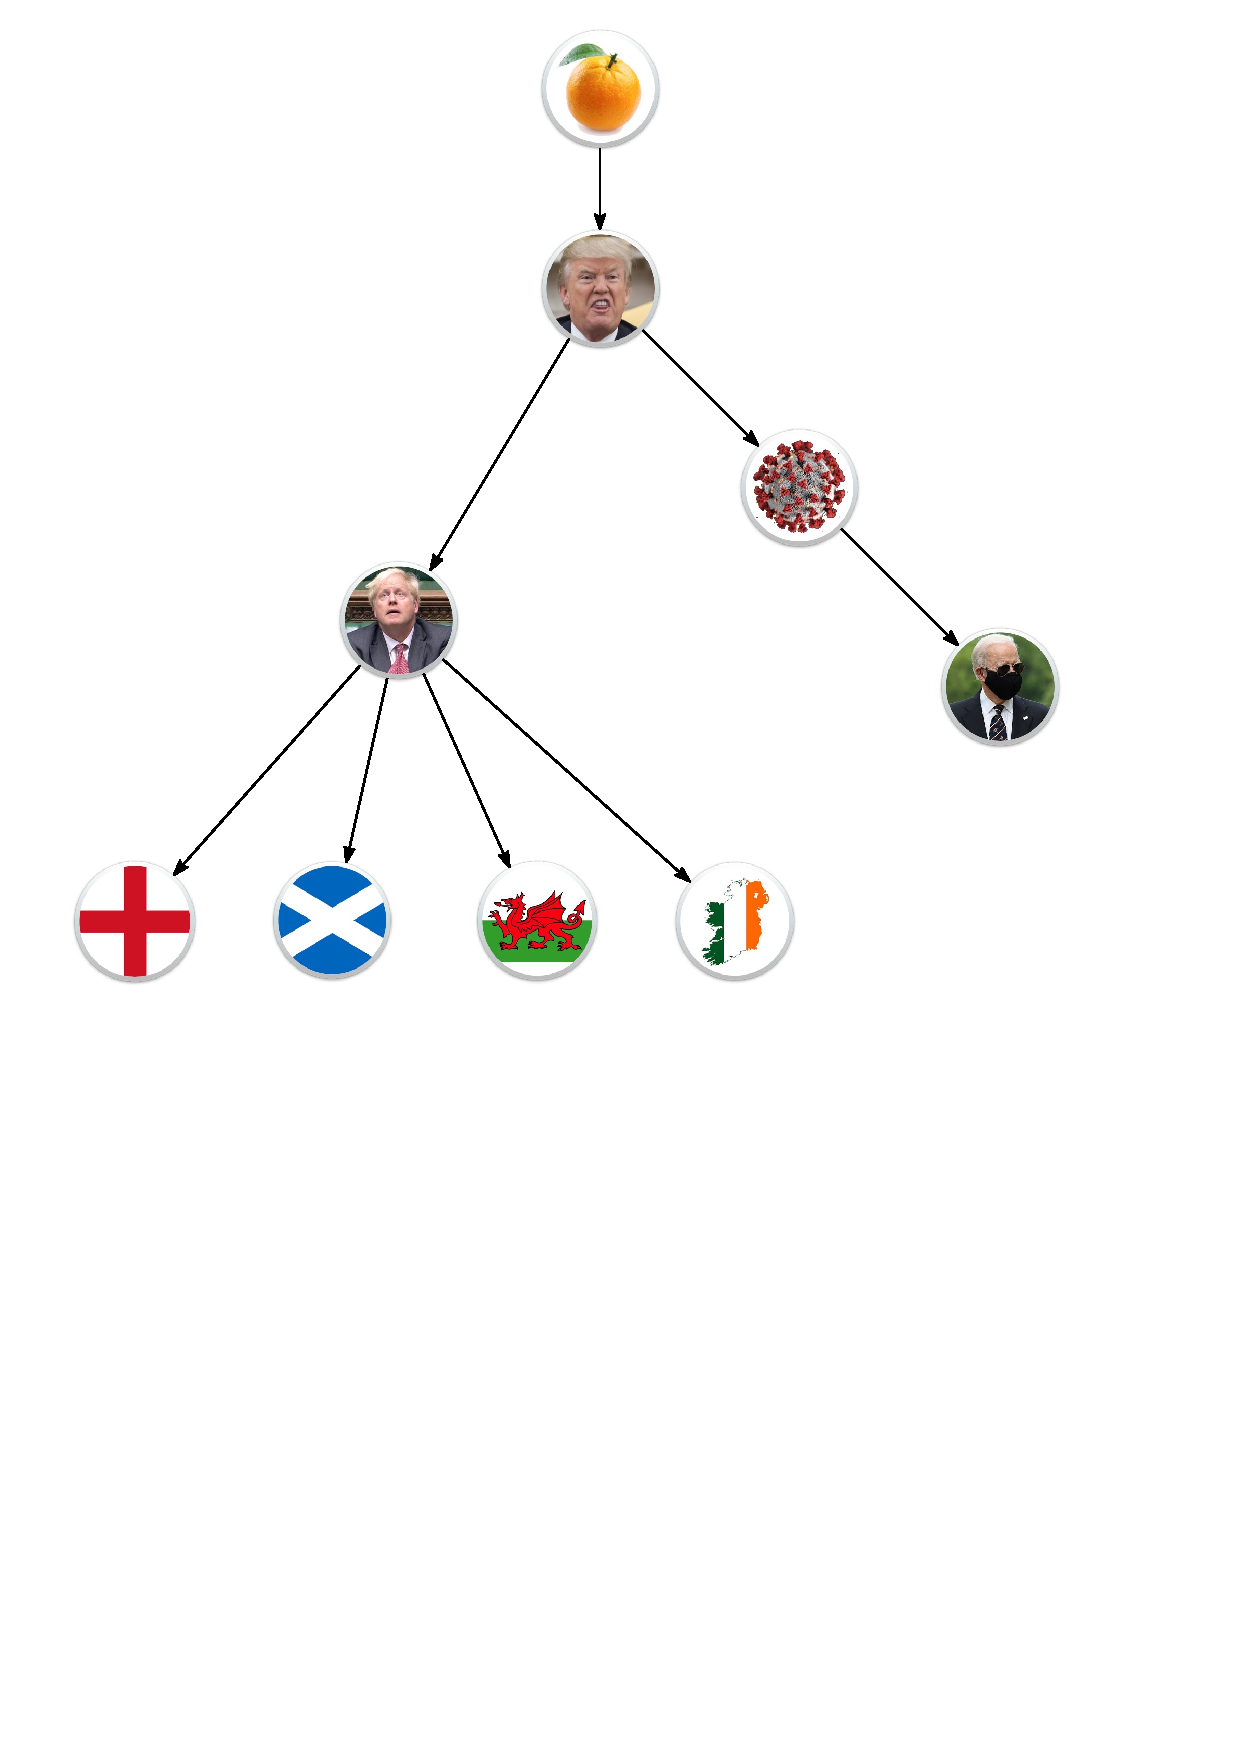
\includegraphics[width=0.5\textwidth, angle=0]{resources/phylogenetic-tree.pdf}
        \end{center}
        \end{block}

    \end{itemize}

\end{frame}

\begin{frame}{Molecular Phylogenetics}

    \begin{itemize}
        \item Sequence of DNA molecules in a genome is represented as a sequence of letters from the four letter alphabet $\Sigma = \{ \texttt{A}, \texttt{C}, \texttt{G}, \texttt{T} \}$.

        \item \emph{Fix for now} an ancestral nucleotide $\texttt{Y} \in \Sigma$; we assume that the following evolution events occur independently:

        $$ \texttt{Y} \overset{ \pi_{\texttt{Y}} \cdot p_{\texttt{A}}^{(\texttt{Y})}  }{\longmapsto}  \texttt{A}, \quad \texttt{Y} \overset{ \pi_{\texttt{Y}} \cdot p_{\texttt{C}}^{(\texttt{Y})}  }{\longmapsto} \texttt{C}, \quad \texttt{Y} \overset{ \pi_{\texttt{Y}} \cdot p_{\texttt{G}}^{(\texttt{Y})}  }{\longmapsto} \texttt{G}, \quad \texttt{Y} \overset{ \pi_{\texttt{Y}} \cdot p_{\texttt{T}}^{(\texttt{Y})}  }{\longmapsto} \texttt{T}, $$ 

        \item So \emph{given} $\texttt{Y}$, we have a joint distribution:
        
        $$ \pi_{\texttt{Y}} \cdot [ p_{\texttt{A}}^{(\texttt{Y})}, p_{\texttt{C}}^{(\texttt{Y})}, p_{\texttt{G}}^{(\texttt{Y})}, p_{\texttt{T}}^{(\texttt{Y})} ] \in \Delta_{3} = \Delta_{4-1}. $$

    \end{itemize}

\end{frame}

\begin{frame}{Example}
    \begin{itemize}
        \item  $\texttt{Y}$ is a hidden variable though; could have been any one of $\texttt{A}, \texttt{C}, \texttt{G}$, or $\texttt{T}$.

        \item For \emph{exactly one given choice} of \texttt{Y}, we had the distribution $\Delta_{3}$; need to consider \emph{all choices} of ancestral nucleotide \texttt{Y}.

        \item Hence we get the mixture model:

        \begin{equation*}
            \begin{split}
                &\Mixt^{4}(\Delta_{3}) \\
                &= \Set{\sum_{ \texttt{Y} \in \{ \texttt{A}, \texttt{C}, \texttt{G}, \texttt{T} \}  } \pi_{\texttt{Y}} \cdot p^{(\texttt{Y})} | \pi \in \Delta_{3},\ p^{(\texttt{Y})} \in \mc{P} \subseteq \Delta_{3}, \text{ for each \texttt{Y}} }.
            \end{split}
        \end{equation*}

    \end{itemize}

    \begin{block}{Question?}
    What is the analogue for mixture models in algebraic statistics?
    \end{block}

\end{frame}

\begin{frame}{Secant Varieties}
    \begin{block}{Answer!}
        Secant\footnote{from \emph{secare}, ``to cut'' in Latin; \emph{c.f. tangō}, ``to touch''.} varieties \cite{BSSSMD2009}!
    \end{block}

    \begin{block}{Definitions}
        \begin{itemize}
        \item Consider two varieties $V, W \subseteq \RR^{k}$. The \emph{join} of $V$ and $W$ is the variety
        $$ \mc{J}(V,W) := \{ \lambda v + (1-\lambda)w : v \in v, w \in W, \lambda \in [0,1] \}. $$

        \item If $V = W$, then this is the \emph{secant variety} of $V$, denoted $\Sec^{2}(V) = \mc{J}(V,V)$. The \emph{$s$-th higher secant variety} is:
        $$ \Sec^{1}(V) := V, \qquad \Sec^{s}(V) := \mc{J}(\Sec^{s-1}(V), V ). $$
        \end{itemize}
    \end{block}

\end{frame}

\begin{frame}{Secant Varieties}
   
    \begin{center}
        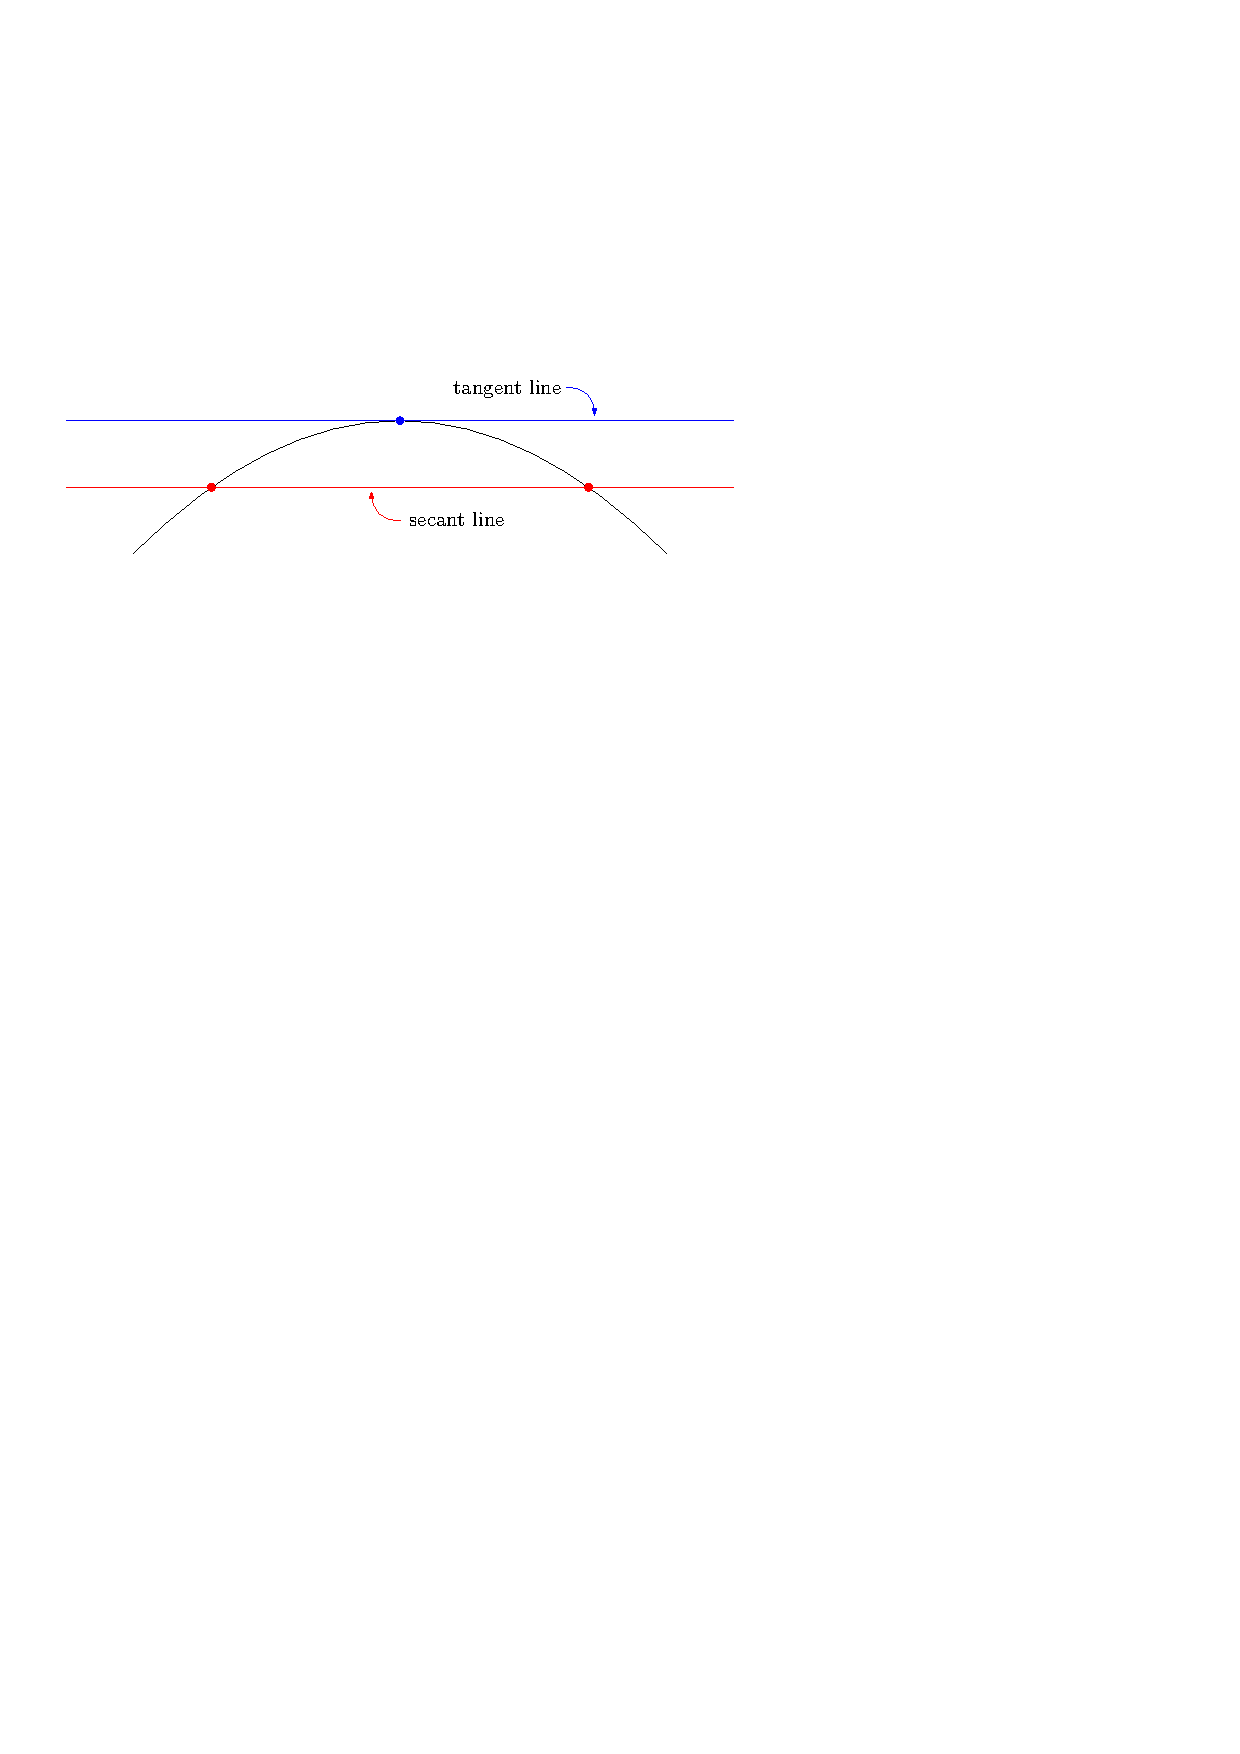
\includegraphics[height=0.25\textwidth, angle=0]{resources/secant-line.pdf}
    \end{center}

    \begin{center}
        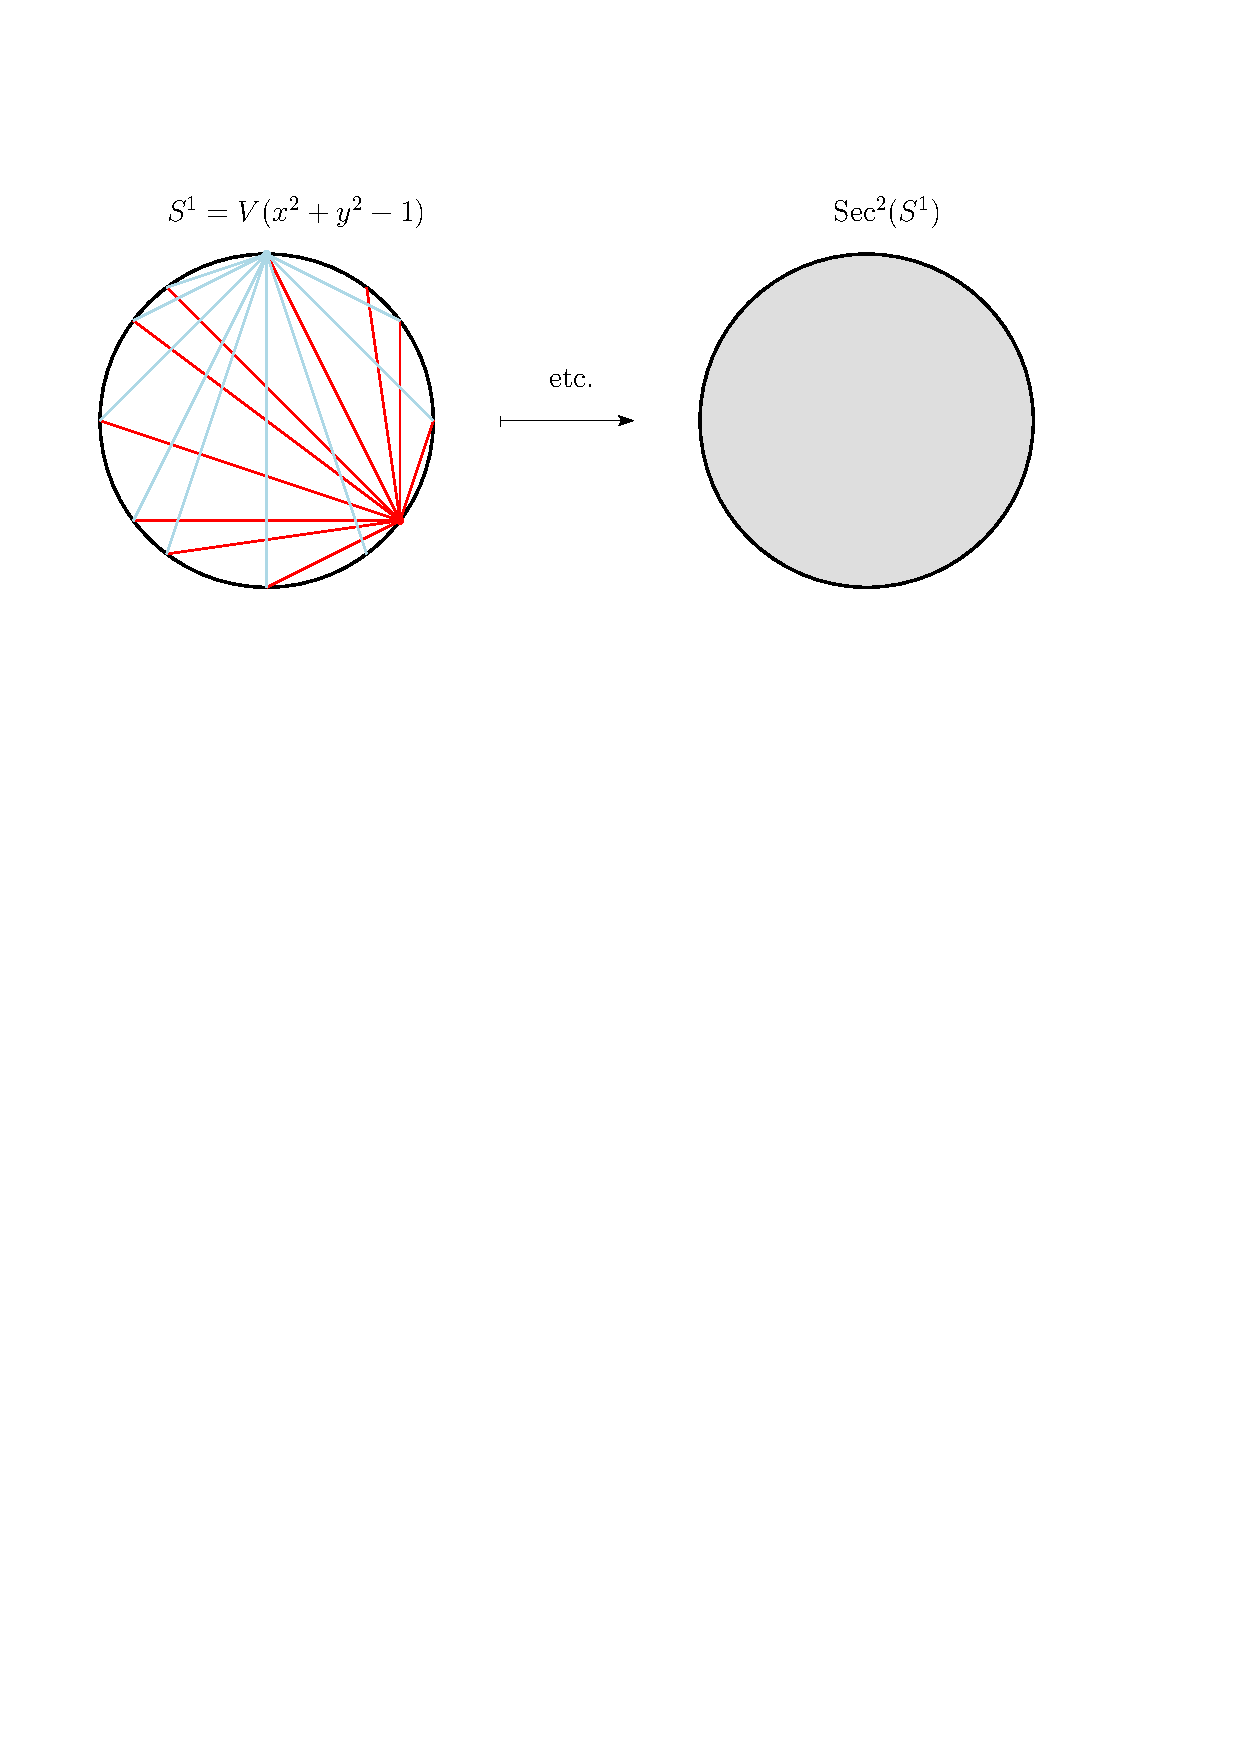
\includegraphics[height=0.35\textwidth, angle=0]{resources/secant-circle.pdf}
    \end{center}

\end{frame}

\begin{frame}{More Complicated Phylogenetic Trees}

    \begin{itemize}
        \item Last example only had one extant species; what about if we had three extant species, all coming from the same ancestor?

    \begin{center}
        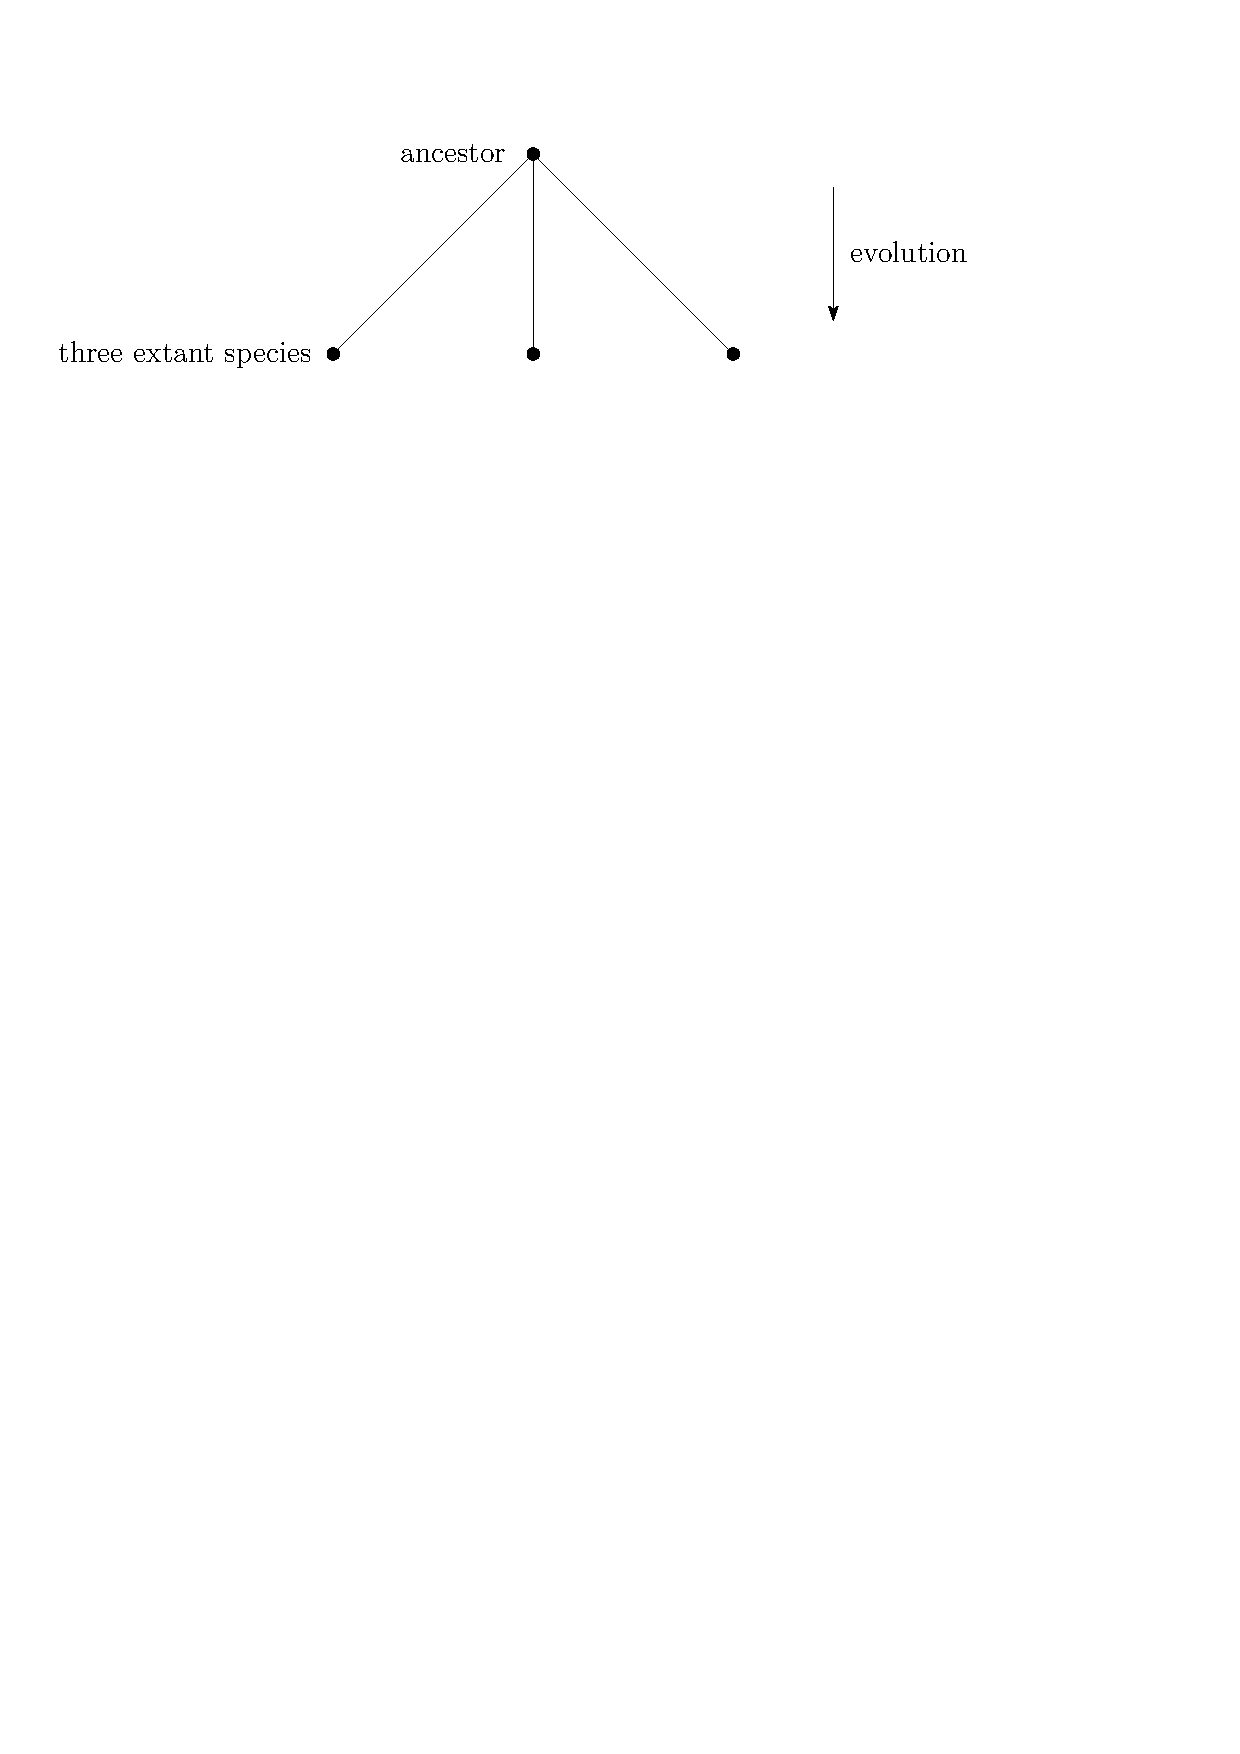
\includegraphics[width=0.6\textwidth, angle=0]{resources/three-extant.pdf}
    \end{center}

    \item Now we have to consider: $\Sec^{4}(\PP^{3} \times \PP^{3} \times \PP^{3})$; or equivalently $\Mixt^{4}(\Delta_{3} \times \Delta_{3} \times \Delta_{3})$.

    \item Finding the minimal set of polynomials defining $\Sec^{4}(\PP^{3} \times \PP^{3} \times \PP^{3})$ once gave rise to a very important application of algebraic statistics...

    \end{itemize}

\end{frame}

\begin{frame}{The \emph{Salmon Problem}}

\begin{block}{Statement}
    \emph{Determine the ideal\footnote{read this as ``set of defining polynomials''.} defining $\Sec^{4}(\PP^{3} \times \PP^{3} \times \PP^{3})$.}
\end{block}

\begin{block}{Prize}
    \begin{itemize}
    \item At an IMA workshop in 2007, Elizabeth Allman stated that she would personally catch and smoke copper river salmon from Alaska for whomever solved this problem. 
    \item Solved in 2010 by Shmuel Friedland \& Elizabeth Gross \cite{SFEG2012} (see \cite{DBLO2011} too for an in-depth discussion).
    \end{itemize}
\end{block}

\end{frame}

\begin{frame}{Revision}

Why $\Sec^{4}(\PP^{3} \times \PP^{3} \times \PP^{3})$ again?

\begin{itemize}
    \item Three independent variables (nucleotides in extant species) $\rightsquigarrow$ three factors in product;
    \item Each independently assumes one value from $\Sigma = \{ \texttt{A}, \texttt{C}, \texttt{G}, \texttt{T} \}$ $\rightsquigarrow$ distribution is a point in $\PP^{3} = \PP^{4-1}$;
    \item The ancestral nucleotide is unknown, but could assume any of the four values in $\Sigma$ $\rightsquigarrow$ mix four such independence models;
    \item The model for the three observed nucleotides is therefore
    \begin{equation*}
            \Sec^{4}(\PP^{3} \times \PP^{3} \times \PP^{3}),\quad \text{\emph{c.f.},} \quad \Mixt^{4}(\Delta_{3} \times \Delta_{3} \times \Delta_{3}).
    \end{equation*}
\end{itemize}
\end{frame}